\section{Visualization of the \gls{lfs} Filters in Triangular Elements}
\label{sec:visualization}
In this section we present visualizations of the effect of the \gls{lfs} filters on a polynomial solution of degree $5$ in a reference triangle.

In the plots that follow, the internal and boundary points are located as shown in Figure \ref{fig:tri_points}.
\epstopdfsetup{update}
\begin{figure}
\centering
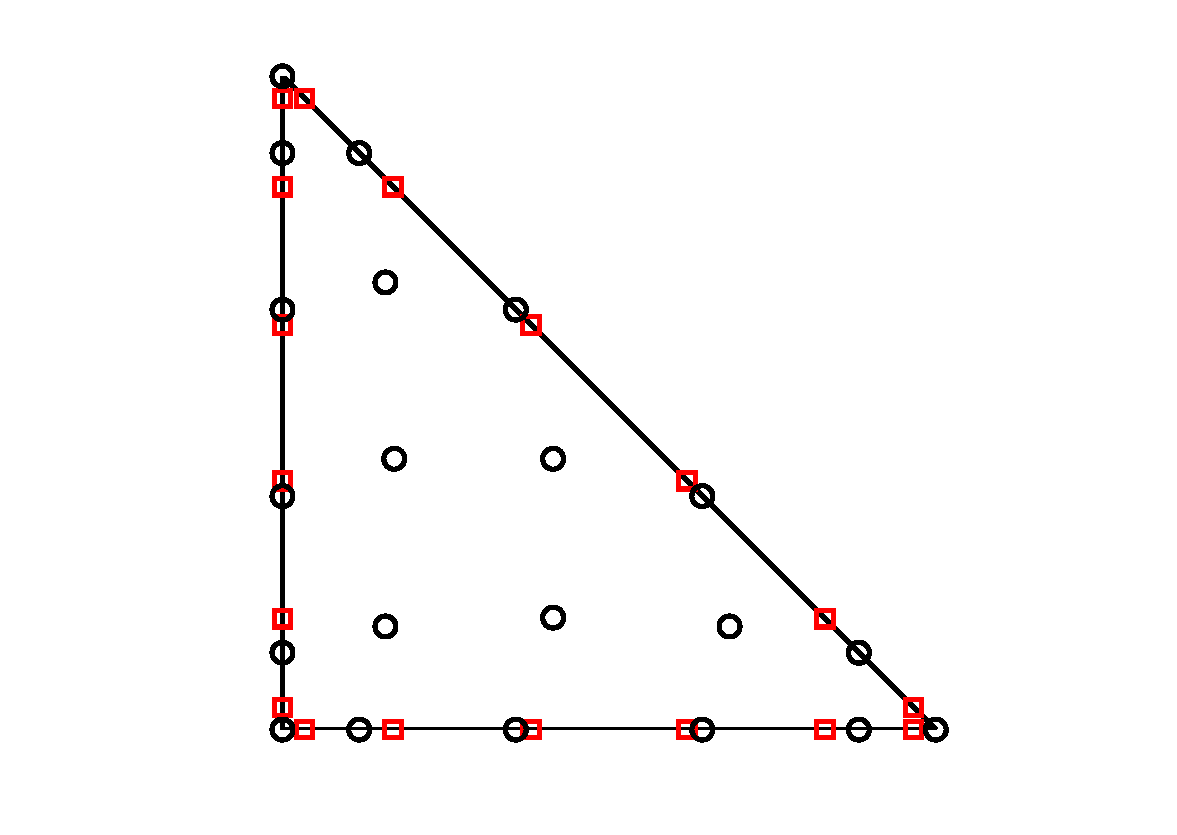
\includegraphics[width = 0.5\textwidth]{\lfsdir/figs/right_triangle_point_locations.eps}
\caption{Internal and boundary points in the reference triangular domain when solution is represented with polynomial of degree $5$ ($p=5$). Black circles represent the internal points. Red squares represent the boundary points.}
\label{fig:tri_points}
\end{figure}

\subsection{Internal Filtering Components}
To illustrate the effect of the internal filtering component, let us filter a solution using matrix $\mat{T}$ exclusively. Figure \ref{fig:internal_filt} shows the result of filtering using a width of $h=10$ in the 2-D sharp-spectral filtering kernel \eqref{item:sharp_spectral} with the modified norm \eqref{eqn:rect_norm}.
\begin{figure}
\centering
\includegraphics[width = 0.5\textwidth]{\lfsdir/figs/internal_effect.eps}
\caption{Solution values after filtering with internal component exclusively, $\vec{\bar{v}} = \mat{T}\vec{v}$, where  ${v_i} = \sin{(k\xi_{i1})} + \cos{(k\xi_{i2})} $, where $k=500$. Hollow black circles show the unfiltered solution at the interior points, transparent colored surface is the polynomial representation of the unfiltered solution, filled black circles show the filtered values of the solution at the interior points, and the meshed surface shows the polynomial representation of the filtered solution.}
\label{fig:internal_filt}
\end{figure}

It can be seen that the polynomial representation of the filtered values is smoother than the polynomial representation of the unfiltered values while maintaining the general shape and curvature.



\subsection{Boundary Filtering Components}
To illustrate the effect of the boundary filtering component, let us filter a solution using matrix $\mat{B}$ exclusively. Figure \ref{fig:boundary_effect} shows the result of filtering. Because only $\mat{B}$ is acting on the solution, the unfiltered values of the solution at the internal points are not plotted. 

We have made all the values of the solution at the boundaries co-planar to illustrate how effectively Condition \ref{item:coplanar} is satisfied. The operation of filtering with $\mat{B}$ does bring the filtered solution closer to a plane if the boundary values are co-planar.

\begin{figure}
\centering
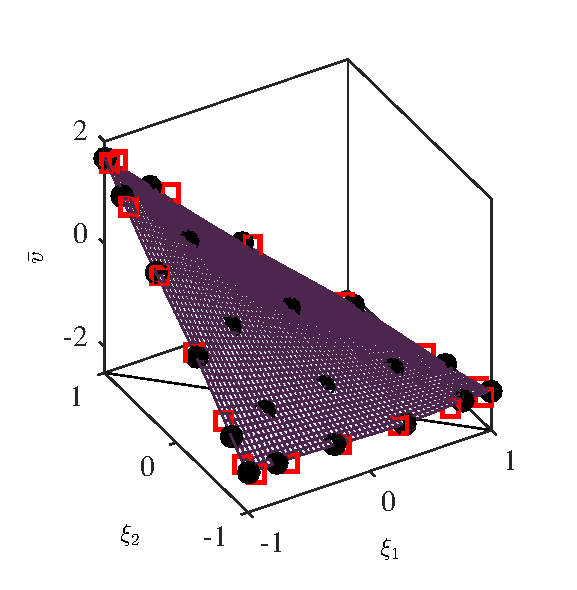
\includegraphics[width = 0.5\textwidth]{\lfsdir/figs/boundary_effect.eps}
\caption{Solution values after filtering with boundary component exclusively, $\vec{\bar{v}} = \mat{B}\vec{v^*}$, where  $\vec{v^*} = a\vec{\xi^*_1} + b\vec{\xi^*_2} + c$ for some constants $a,b,c$. Red squares show the values of the solution at the boundaries, filled black circles show the filtered values of the solution at the interior points, and the meshed surface shows the polynomial representation of the solution.} 
\label{fig:boundary_effect}
\end{figure}

Figure \ref{fig:boundary_effect_oscillatory} illustrates how the boundary filtering component would behave in the case the boundary values are not coplanar. It is interesting to note that close to the corner $(\xi_1,\xi_2) = (-1,1)$, two boundary points with different values are close to an internal point. The value  of the filtered solution close to those boundary points assumes a value that is close to the average of the two.

The polynomial interpolation of the filtered interior values shows that the closer an interior point is to a boundary point, the more it will be influenced by such boundary point. This causes the filtered values close to the boundaries to get closer to the boundary values. This suggests that the boundary filtering component does in fact help in bringing the solution closer to satisfying the boundary conditions while diminishing oscillations within the element.

\begin{figure}
\centering
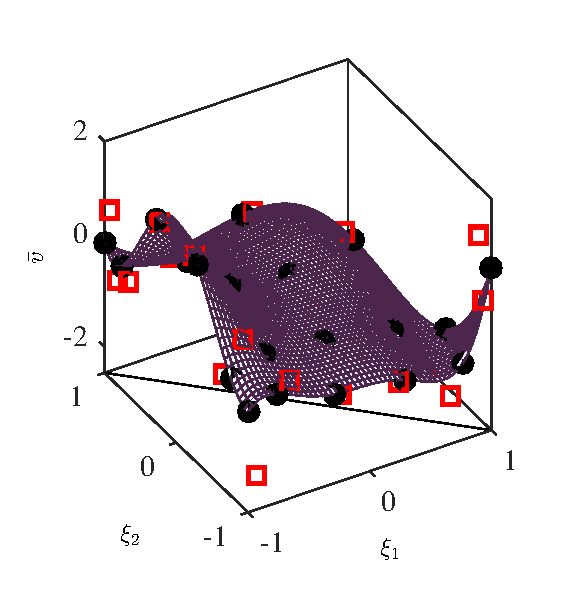
\includegraphics[width = 0.5\textwidth]{\lfsdir/figs/boundary_effect_oscillatory.eps}
\caption{Solution values after filtering with boundary component exclusively, $\vec{\bar{v}} = \mat{B}\vec{v^*}$, where   ${v_i^*} = \sin{(k\xi^*_{i1})} + \cos{(k\xi^*_{i2})} $, $k=500$. Red squares show the values of the solution at the boundaries, filled black circles show the filtered values of the solution at the interior points, and the meshed surface shows the polynomial representation of the solution.} 
\label{fig:boundary_effect_oscillatory}
\end{figure}

\subsection{Filtered Solutions}
No filtering component is used solely by itself. The factor $\alpha$ in Equation \ref{eqn:filter_form} determines how much weight to give to each component. Figure \ref{fig:filtered_solutions} illustrates the effect of the boundary values on a fully filtered solution, when $\alpha = 0.8$.

The internal filtering component reduces oscillations, while the boundary filtering component brings the interior values closer to the boundary values. By placing the boundary values on different planes, this effect becomes more evident.

\begin{figure*}
\hspace{-1cm}
\subfloat[$\beta = -0.75$\label{fig:filt_neg}]{%
\includegraphics[width=0.5\textwidth]{\lfsdir/figs/filter_tilt_neg.eps}
}
\hfill
\subfloat[$\beta = 0.75$\label{fig:filt_pos}]{%
\centering
\includegraphics[width=0.5\textwidth]{\lfsdir/figs/filter_tilt_pos.eps}
}
\caption{Solution values after filtering with both internal and boundary components, $\vec{\bar{v}} = \alpha\mat{T}\vec{v} + (1-\alpha)\mat{B}\vec{v^*}$, where $\alpha = 0.8$, ${v_i} = \sin{(k\xi_{i1})} + \cos{(k\xi_{i2})} $, $k=500$, $\vec{v^*} = \beta (-\vec{\xi^*_1} + \vec{\xi^*_2})$. Hollow black circles show the unfiltered solution at the interior points, transparent colored surface is the polynomial representation of the unfiltered solution, filled black circles show the filtered values of the solution at the interior points, hollow red squares show the value of the solution at the boundary points, and the meshed surface shows the polynomial representation of the filtered solution.}
\label{fig:filtered_solutions}

\end{figure*}